\chapter{Literature Survey}
%wide context
%detailed context
%recent work 
%    critically assess previous work
%questions and issues that have not yet been answered



\section{Speech Prosody}
In linguistics, the term prosody refers to the use of suprasegmental features such as rhythm and intonation to convey sentence-level pragmatic meanings \citep{Jurafsky2008}. Most of the previous study focuses on the prosodic structure, prosodic prominence, tune and the use of features including pitch, energy and duration \citep{Pierrehumbert1980,Pierrehumbert1990,Pierrehumbert2015,Hirschberg2002}. Prosodic cues have been applied to many fields of speech and language processing, especially speech synthesis, automatic summarization and emotion detection in speech utterances \citep{Hong2015}. Recently, researchers explored vector representation of words based on speech and its prosodic features \citep{He2016, Chung2018}, a similar approach as the widely used word embedding technique "word2vec" in Natural Language Processing.     

Analysis of prosody
methodological 
introspective transcription

acoustic transcription
Tones and Break Indices (ToBI) 
directly observable,
example-based work
questioned: hypothetical nature

hypothesis testing

\subsection{Prosodic analysis}
Prosodic analysis aims to compute an abstract representation of the prosodic prominence, structure and tune of the spoken utterance.

\subsubsection{Prosodic Structure}
Similar to syntactic structure, speech utterances have a structure that some words group naturally together and form a boundary or break. there is a term to describe prosodic structure called prosodic phrasing. A spoken sentence is divided into intonational phrases, for instance, separated by commas, and even smaller units called intermediate phrases. 

Prososic phrasing is of great use in tasks such as speech synthesis. Automatic phrase boundary detection can be regarded as a classification problem. 

\subsubsection{Prosodic Prominence}
When a speaker says some words in a lower or louder voice or in a high pitch, the listener seems to feel these words are more prominent or important. Pitch accent is the linguistic marker used to denote a prosodic prominence, which is related to stress. Most of the content words are accented whereas function words tend not to bear pitch accent. Generally speaking, more informative words (for example new words or unexpected words) are more likely to bear accent \citep{Jurafsky2008, Ladd2008}.

In practice, prominence is usually categorised into four levels: emphatic accent, pitch accent, unaccented, and reduced. Given the close relation between prosodic prominence and word importance, the description and application of prominence requires semantic knowledge. Features such as TF-IDF, part-of-speech and accent ratio are usually adopted to predict accents.

\subsubsection{Tune}
The tune of an utterance is the rise and fall of its $F_0$ over time. The typical tunes in English are a rise of the voice at the last word in a yes-no question and a drop at the end of a statement. The former is called the question rise and the latter the final fall. 

The tune is a useful facility to express meaning and emotions. It can be inferred from the tune contour that whether the speaker is surprised or in a contradiction. For a long time, most of the systems are only able to distinguish two or three tunes yet more and more work emerges on this topic.

\subsection{Tone and Break Indices Model: ToBI}
ToBI (Tone and Break ToBI Indices) is the dominant linguistic model for describing prosodic features in American English speech utterance \citep{Silverman1992, Pitrelli1994}. It models boundaries, prominence, tune based on the 4 boundary tones and 5 pitch accents shown in the following table.

%(insert table here)
\begin{figure}[ht]
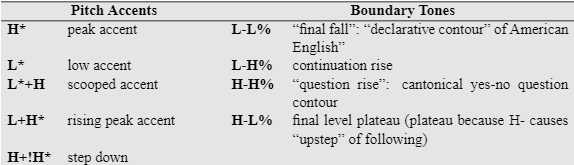
\includegraphics[width=15cm]{figures/ToBI_1.png}
\caption{The accent and boundary tones labels from the ToBI transcription system Reproduced from D. Jurafsky and J.H. Martin, 2nd\_ed\_draft: Speech and Language Processing with the permission of the copyright owner.}
\label{fig:ToBI1}
\end{figure}

In ToBI, an input utterance is represented by a sequence of intonational phrases and intermediate phrases. The intonational phrases end in one of the four boundary tones which describe the tune. Each word in the utterances will be assigned a pitch accent of the five types. Furthermore, ToBI adopts a separate break index tier to distinguishes four levels of phrasing: break index4-intonational phrase; break index 3-intermediate phrase; break index2-disjuncture or pause; break index 1--medial word boundaries \citep{Hirschberg2002}.

%(insert figure here)

\begin{figure}[ht]
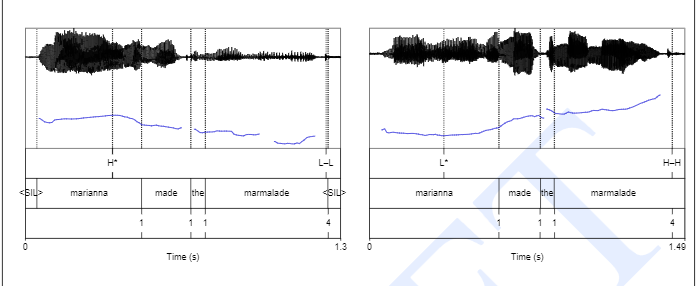
\includegraphics[width=15cm]{figures/ToBI_2.png}
\caption{An example of ToBI discription, Reproduced from D. Jurafsky and J.H. Martin, 2nd\_ed\_draft: Speech and Language Processing with the permission of the copyright owner.}
\label{fig:ToBI2}
\end{figure}

One goal of ToBI is to display the link between meanings and pitch accents. With the Praat program, we are able to visualise the tone, orthographic, and phrasing tiers of a ToBI transcription. In (a), the word Marianna is spoken with a high $H^*$ accent, and the sentence has the declarative boundary tone L-L\% whereas in (b) the same word is spoken with a low $L^*$ accent implying a surprise emotion. In addition, boundary tone H-H\% in (b) follows the yes-no question pattern \citep{Pitrelli1994, Jurafsky2008}. 


\subsection{Speech to vector representation}
Similar to word-embedding for text e.g., word2vec \citep{Mikolov2013}, various researchers have investigated encoding semantic properties of a word directly from speech \citep{Chung2018}. 

\citet{Brenier2005} found that pitch and energy features have been effective for intonation modelling and speech emphasis detection. It was shown by \citet{Tamburini2003} that RMS energy from a mid-range frequency band (500-2000 Hz) is useful for detecting prominence of syllables. The number of syllables spoken in a word can also be estimated using the methodology of \citet{DeJong2009}. Other spoken-lexical features have also been proved useful including the duration of a word, syllable and silence, the position of a word in the utterance and etc. 

Apart form pitch, energy and lexical features, voicing features is the area where more and more researches appear. The spectral-tilt measure represents the difference between the amplitudes of the first harmonic (H1) and the second harmonic (H2) in the Fourier Spectrum. It is proved by \citet{Keating2006} that spectral-tilt is effective in characterizing glottal constriction, a factor in distinguishing voicing characteristics. There exists other voicing measures, for example, Harmonics-to-Noise Ratio and Voiced Unvoiced Ratio.

\citet{Kafle2019} developed a model to learn a word-level representation from prosodic features at a sub-word level for the task of importance prediction in spoken dialogue. Using Praat they extracted 30 features in total: 3 voicing features, 6 spoken-lexical features, 10 pitch-related features and 11 energy features. These features also got speaker-normalized (ZNORM).


%http://ec-concord.ied.edu.hk/phonetics_and_phonology/wordpress/learning_website/chapter_1_introduction_new.htm#1.2.1

%\section{applications}
%Previous researchers have modeled prosodic
%cues in speech for various applications (Tran et al., 2017; Brenier et al., 2005; Xie et %al., 2009). 
%
%For instance, in automatic prominence detection, re- searchers predict regions of speech %with relatively more spoken stress (Wang and Narayanan, 2007; Brenier et al., 2005; %Tamburini, 2003). Identifi- cation of prominence aids automatically identify- ing content %words (Wang and Narayanan, 2007), a crucial sub-task of spoken language understand- ing %(Beckman and Venditti, 2000; Mishra et al., 2012). 
%
%Moreover, researchers have investigated modeling prosodic patterns in spoken messages to %identify syntactic relationships among words (Price et al., 1991; Tran et al., 2017). In %particular, (2017) demonstrated the effectiveness of speech- based features in improving %the constituent pars- ing of conversational speech texts. In other work, researchers %investigated prosodic events to iden- tify important segments in speech, useful for pro- %ducing a generic summary of the recordings of meetings (Xie et al., 2009; Murray et al., %2005).

\section{Word Importance}
Researchers in Psychology have used eye-trackers to study reading behavior. They found that readers tend to skip words, gaze on a word or glance back at previous words instead of reading very word in a text sequentially. It indicates that some words seem more important than others and words which are often skipped over by the readers tend to be shorter and more predictable \citep{Rayner2011}. 

\subsection{Word importance estimation}

Prior research on identifying and scoring important words in a text basically focused on the task of keyword extraction and document automatic summarisation. Metrics of word importance been used include Term Frequency x Inverse Document Frequency (TF-IDF) weighting \citep{HaCohen-Kerner2010}, word co-occurrence probability estimation \citep{Y.MATSUO2004} as well as linguistic features that investigated by supervised learning methods \citep{Liu2011, I.Sheeba2012}. In the study of word importance for spoken sentences, \citet{Kafle2018} have developed a corpus with word importance being labelled by human annotators using a deliberated metrics framework.

\subsection{TF-IDF}
Term Frequency - Inverse Document Frequency (TF-IDF) is a widely used metric in information retrieval which reflects the term weight or importance of a word to the corpus. Given a corpus with $D$ documents, the TF of a word $N_w$ means the number of appearance of a word $w$ in a particular document $d$. Document Frequency indicates that there are $k$ documents in the corpus, which contain the certain word $w$. In practice, we use the inverse document frequency times term frequency to capture the semantic importance of a word in the context of that corpus \citep{Jurafsky2008}.

\begin{equation}
TF*IDF(w) = N_w \times \log(\frac{D}{k})
\label{eq:tf-idf}
\end{equation}

\subsection{Perplexity}
Perplexity (denoted by $PP$ for short) is the most common evaluation metric to test how well a statistical language models matches a test corpus.  For a test set $W = {w_1, w_2, \cdots, w_N}$ where $w_i$ is a sentence in the set, the perplexity is the probability of the test set, normalized by the number of words \citep{Jurafsky2008}:

\begin{equation}
PP(W) = P(w_1, w_2, \cdots, w_N)^{-\frac{1}{N}}\\
= \sqrt[N]{\prod_{i=1}^{N} \frac{1}{P(w_i|w_1, w_2,\cdots, w_{i-1})}}
\label{eq:perplexity}
\end{equation}

It is assumed that a better language model will assigns a higher probability, or higher maximum likelihood to a sentence of the test set hence the perplexity will be lower. Furthermore, this model will perform better in word prediction.

\subsection{RIT annotation}
The Linguistic and Assistive Technologies Laboratory at the Rochester Institute of Technology (RIT) released an open word importance annotation corpus in 2017. They augumented the transcripts of the famous the Switchboard conversational dialogue corpus \citep{Godfrey1992} based on the work of the Institute for Signal and Information Processing (ISIP). A pair of annotators have assigned word importance scores to Switchboard transcripts. By September 2017, over 25,000 tokens have been annotated including the overlap of approximately 3,100 tokens. 

\citet{Kafle2018} defined word importance as a continuous scale from 0.0 (not important
at all to the meaning of the utterance) to 1.0 (very important). The annotator has been given a rating scheme which specifies the scoring criteria and they should also consider how much the meaning of the utterance be changed if a word has been deleted. Here is an example showing how the scoring system works.

\begin{figure}[ht]
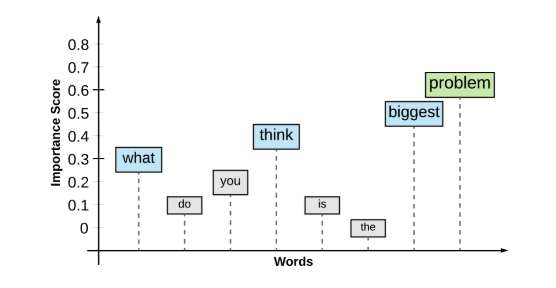
\includegraphics[width=15cm]{figures/word.png}
\caption{An example of RIT annotation, Reproduced from S. Kafle and M. Huenerfauth, 2018, A Corpus for Modeling Word Importance in Spoken Dialogue Transcripts, with the permission of the copyright owner.}
\label{fig:word}
\end{figure}



%While this conceptualization of word importance as a keyword-extraction problem has led to positive results in the %field of text summarization (Litvak and Last, 2008; Wan et al., 2007; Hong and Nenkova, 2014), this approach may not %generalize to other applications.
%
%For instance, given the sometimes meandering nature of topic transition in spontaneous speech dialogue (Sheeba and %Vivekanandan, 2012), applications that process transcripts of such dialogue may benefit from a model of word %importance that is more local, i.e. based on the importance of a word at sentential, utterance, or local dialogue %level, rather than at a document- level. 
%
%Furthermore, the dyadic nature of dialogue, with interleaved contributions from multiple speakers, may require %special consideration when evaluating word importance. In this paper, we present a corpus with annotation of word %importance that could be used to support research into these complex issues.


\section{Data}
Choosing appropriate spoken data is of vital importance of this experimental project. Prosodic feature extraction requires huge clearly articulated utterance in the general domain. An open utterance corpus with transcripts is preferred for the convenience of building language models. Considering these two, the author has chosen the Switchboard corpus as data source and a widely used software called Praat for feature extraction.

\subsection{Switchboard corpus}
The Switchboard corpus is a large multi-speaker database of conversational speech. It consists of recordings of approximately 260 hours of telephone conversations among 543 speakers (241 female, 302 male) from across the United States. In 2003, the Institute for Signal and Information Processing (ISIP) released written transcripts for the entire corpus with a complete vocabulary list and automatic word alignment timing corresponding to the original audio files. \citet{Kafle2018} in the Rochester Institute of Technology (RIT) released an free-to- download augumented version of ISIP transcripts for word-importance modelling. 

\subsection{Feature extraction tool: Praat}
Praat \citep{PaulBoersma&DavidWeenink2018} is a freeware program for the analysis and reconstruction of acoustic speech signals. The user is able to analyze, synthesize, manipulate speech and plot pictures for visualisation in papers. It was designed, and continues to be developed, by Paul Boersma and David Weenink of the University of Amsterdam. Praat is available for most platforms. The clear visual presentation of operational procedures and introduction to acoustic knowledge are provided to facilitate the users in linguistic research.

Some of its functionalities include:
\begin{itemize}
    \item generate waveforms, wide and narrow band spectrograms, intensity contour and pitch tracks;
    \item get information about pitch, intensity, formants, pulses and etc;
    \item enhance certain frequency regions; segment and label words, syllables, or individual phonemes;
\end{itemize}

\begin{figure}[ht]
\center
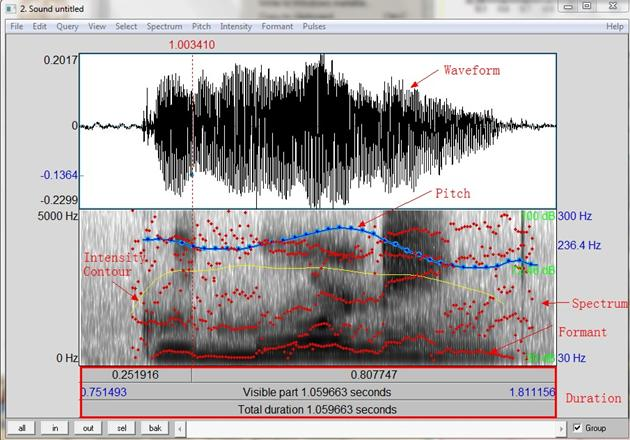
\includegraphics[width=10cm, scale=0.7]{figures/Praat.jpg}
\caption{Speech analysis sofware Praat, from http://ec-concord.ied.edu.hk/}
\label{fig:praat}
\end{figure}

\section{Spearman Rank Order Correlation Coefficient}
pearson, spearman, kadel?
spearman is suitable
equation
numpy faster than pandas


%LM with prosodic features:
%Sub-word to Word-level Representation 
%The acoustic features listed above were extracted from a 50-ms sliding window over each %word re- gion with a 10-ms overlap. In our model, each word was represented as a sequence %of these sub- word features with varying lengths, as shown in Figure 2. To get a feature %representation for a word, we utilized a bi-directional Recurrent Neu- ral Network (RNN) %layer on top of the sub-word features. The spoken-lexical features were then concatenated %to this word-level feature representa- tion to get our final feature vectors. For this %task, we utilized Gated Recurrent Units (GRUs) (Cho et al., 2014) as our RNN cell, rather %than LSTM units, due to better performance observed during our initial analysis.
%5

%\section{A Section that Contains Some References}
%
%According to seminal research by \cite{Reference1}, lorem ipsum dolor sit amet.  However, %this result was already known in the 1990s \citep{Reference2,Reference3}.  % Note the use %of \cite{} and \citep{}
%
%
%\section{A Section that Contains Some Maths}
%
%\lipsum  % Replace with your text
% 
%\begin{equation}
%M = \frac{1}{T}\sum_{t=1}^{T} e(t) / \max_{t}[e(t)]
%\label{eq:equation}
%\end{equation}
%
%\lipsum  % Replace with your text
%
%This is shown in Equation \ref{eq:equation} and is repeated here $M = %\frac{1}{T}\sum_{t=1}^{T} e(t) / \max_{t}[e(t)]$.
%
%
%\section{A Section that Contains a Figure}
%
%\lipsum  % Replace with your text
%
%\begin{figure}[ht]
%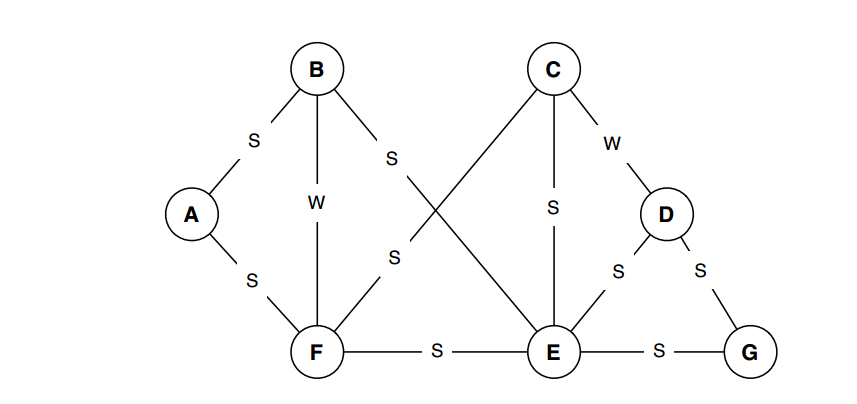
\includegraphics[width=15cm]{figures/figure1.png}
%\caption{A simple figure in \LaTeX. Reproduced from http://tinyurl.com/nqtrlj5 with the %permission of the copyright owner.}
%\label{fig:graph}
%\end{figure}
%
%\lipsum  % Replace with your text
%
%See Figure \ref{fig:graph}.
%
%
%\section{A Section that Contains a Table}
%
%\lipsum  % Replace with your text
%
%\begin{table}[ht]
%\center
%\begin{tabular}{cc|c}
%A & B & A XOR B\\
%\hline
%0 & 0 & 0\\
%0 & 1 & 1\\
%1 & 0 & 1\\
%1 & 1 & 0\\
%\end{tabular}
%\caption{A simple table in \LaTeX.}
%\label{tab:xor}
%\end{table}
%
%\lipsum  % Replace with your text
%
%This is shown in Table \ref{tab:xor}.
%
%
%\section{Summary}
%
%\lipsum  % Replace with your text
